\documentclass[10pt,a4paper]{article}

\usepackage[spanish]{babel}
\usepackage[utf8]{inputenc}
\usepackage{geometry}
\usepackage{url}
\usepackage{amsmath}
\usepackage{graphicx}
\usepackage{float}
\usepackage{listings}
\usepackage{color}
\usepackage{multicol}
\definecolor{grey}{rgb}{0.8,0.8,0.8}
\usepackage{listings}
\usepackage{color,soul}
\usepackage{caption}
\usepackage{subcaption}
%\usepackage{bibtex}


% Macros
% #1 : Path of image. eg : window/aWindow.png
% #2 : Caption of image. eg : a caption
% #3 : Width of image in centimeters. eg : 15
% #4 : Height of image in centimeters. eg : 20
% 
% example : \presentgrafic{window/aWindow.png}{caption}{15}{20}
\newcommand{\presentgrafic}[4]{
\begin{figure}[H]
\centering
\includegraphics[width=#3cm, height=#4cm]{#1}
\caption{#2}
\label{fig:my_label}
\end{figure}
}


\begin{document}

\begin{titlepage}

\newcommand{\HRule}{\rule{\linewidth}{0.5mm}} % Defines a new command for the horizontal lines, change thickness here

\center % Center everything on the page

\textsc{\LARGE Facultad de Ingeniería - UBA}\\[1.5cm]
\textsc{\Large Organización de Datos 75.06}\\[0.5cm]
\textsc{\large Trabajo Práctico: Diseño}\\[0.5cm]

\HRule \\[0.4cm]
{ \huge \bfseries Fine Food Reviews}\\[0.4cm]
\HRule \\[1.5cm]

\begin{minipage}{0.5\textwidth}
\begin{flushleft} \large
\emph{Integrantes:}\\
Agustina \textsc{Barbetta} \textit{96528}\\
Santiago \textsc{Lazzari} \textit{96735}\\
Luciano \textsc{Mintrone} \textit{95463}\\
Manuel \textsc{Porto} \textit{96587}\\
\end{flushleft}
\end{minipage}
~
\begin{minipage}{0.4\textwidth}
\begin{flushright} \large
\emph{ }\\
\texttt{agustina.barbetta@gmail.com}\\
\texttt{santilazzari1994@gmail.com}\\
\texttt{lucianomintrone@gmail.com}\\
\texttt{manu.porto94@gmail.com}\\
\end{flushright}
\end{minipage}\\[2cm]

{\Large \texttt{Rayo Privatizador}}\\[2cm]

\selectlanguage{spanish}
{\large \today}\\[3cm]

\begin{abstract}
En el presente trabajo se analiza un set de datos con reseñas de productos y se estudian distintas estrategias para desarrollar un modelo capaz de predecir el puntaje de las mismas.
\end{abstract}

%\includegraphics{Logo}\\[1cm]

\vfill % Fill the rest of the page with whitespace

\end{titlepage}


\iffalse

\title{\textbf{Trabajo Práctico:\\  Fine Food Reviews}}

\author{Agustina Barbetta, \textit{Padrón Nro. 96528}\\
        \texttt{agustina.barbetta@gmail.com}\\\\
        Santiago Lazzari, \textit{Padrón Nro. 96735}\\
        \texttt{santilazzari1994@gmail.com}\\\\
        Luciano Mintrone, \textit{Padrón Nro. 95463}\\
        \texttt{lucianomintrone@gmail.com}\\\\
        Manuel Porto, \textit{Padrón Nro. 96587}\\
        \texttt{manu.porto94@gmail.com}\\
        \\[2.5ex]
        \normalsize{2do. Cuatrimestre de 2016}\\
        \normalsize{75.06 Organización de Datos}\\
        \normalsize{Facultad de Ingeniería, Universidad de Buenos Aires}\\
       }


\begin{document}
\date{19 de Septiembre de 2016}

\maketitle

\thispagestyle{empty}
\begin{abstract}
cosas
\end{abstract}

\pagebreak

\fi

\tableofcontents

\pagebreak

\section{Introducción}
El objetivo de este trabajo es predecir la cantidad de estrellas de un review en base a los datos del mismo.\\
En el presente informe, se parte de un análisis de los sets de datos dados, es decir, todo lo relacionado con las distintas métricas, para luego investigar los potenciales algoritmos a utilizar en la búsqueda de una solución definitiva. En la sección \textbf{Investigación} se presenta cada algoritmo individualmente, con una explicación del funcionamiento del mismo, sin compararlos entre sí. Más adelante se relatan los modelos utilizados hasta el momento junto con sus resultados.
Finalmente, en la sección de \textbf{Modelo a implementar}, se presentará la solución elegida justificando el por qué de nuestra decisión y su preferencia sobre los otros algoritmos.  

\section{Pre-procesamiento}

Antes de comenzar el análisis, escribimos un \textit{script} para; eliminar HTML markup, caracteres especiales, números y pasar a minúscula todo el texto correspondiente a los campos \texttt{Summary} y \texttt{Text} de cada \textit{review}.

Además, utilizamos la biblioteca \texttt{nltk}\footnote{Natural Language Toolkit: http://www.nltk.org/} para obtener versiones sin \textit{stopwords} y con \textit{stemming} de los sets de datos.

Como no utilizaremos todos los pasos de este proceso para los diferentes tipos de análisis, los enumeramos en la siguiente lista a la cual haremos referencia en las próximas secciones.
\begin{enumerate}
    \item Eliminación de HTML
    \item Eliminación de caracteres especiales
    \item Eliminación de caracteres numéricos
    \item Pasaje a lower case
    \item Eliminación de stopwords
    \item Stemming
\end{enumerate}

Para este trabajo, buscamos extraer información a partir de diferentes textos. El motivo de este pre-procesamiento es filtrar de los documentos a aquellas palabras que no provean información relevante, así como también, llevar todas las palabras con un significado equivalente a un mismo formato.

\section{Análisis}

\subsection{Utilidad de los campos del set}
Uno de los primeros análisis realizados consistió en evaluar la utilidad de los campos presentes en el set. A continuación se enumeran todos los campos existentes:

\begin{enumerate}
    \item \textbf{Id:} El Id que identifica a cada review
    \item \textbf{ProductId:}  El Id del producto
    \item \textbf{UserId:} El Id del usuario
    \item \textbf{ProfileName:} El nombre del usuario
    \item \textbf{HelpfulnessNumerator:} El numerador indicando la cantidad de usuarios que juzgaron al review como util
    \item \textbf{HelpfulnessDenominator:} El denominador indicando la cantidad de usuarios que evaluaron si el review fue útil o no
    \item \textbf{Prediction:}  La cantidad de estrellas del review. Valor entero entre 1 y 5.
    \item \textbf{Time:} Un timestamp para el review
    \item \textbf{Summary:} Un resumen del review
    \item \textbf{Text:} Texto del review
\end{enumerate}

En principio, los campos ``Id'', ``ProfileName'' y ``Time'' no fueron considerados de utilidad. El primero porque su única función es la de identificar cada review y no aporta ningún tipo de información sobre la misma. El segundo no es necesario ya que se cuenta con el Id del usuario, además de que el nombre de perfil de un usuario no necesariamente es único, no siendo el caso de su Id.  Por último, el campo ``Time'' también fue descartado ya que no se encontró ninguna razón por la cual el timestamp de una reseña pueda ser de utilidad para predecir el puntaje de la misma.

El Id del usuario podría aportar información útil ya que, junto con sus puntuaciones de productos es posible predecir como suele calificar los productos. Sin embargo, si se realiza un análisis sencillo sobre el set, se advierte que le promedio de reviews por usuario es demasiado bajo (\texttt{2 reviews/usuario}) y que solo el 17,7\% de los usuarios se encuentra por encima de este valor. Esto no quiere decir que el campo ``UserId'' deba ser descartado, pero en caso de utilizarse se deberá tener en cuenta lo recién expuesto para filtrar a aquellos usuarios con una cantidad de reviews insuficientes para poder aportar información útil al modelo.

Una situación similar ocurre con los campos ``HelpfulnessNumerator'' y ``HelpfulnessDenominator''. En principio, esta información podría ser de utilidad para asignar pesos a las distintas reseñas, es decir, se le daría mas importancia a aquellas reviews que hayan sido útiles para los usuarios y se le quitaría importancia a aquellas que no lo sean. Además de que este razonamiento no necesariamente implique un beneficio al modelo ya que, el hecho de que una reseña sea útil para un grupo de usuarios no implica que lo sea para el algoritmo utilizado, estos campos presentan la misma problemática que el ``UserId''. En el campo ``HelpfulnessDenominator'' que indica a cuántos usuarios les pareció útil o no una reseña se encuentra un valor promedio de 2,24. Además, solo el 21,8\% de los reviews se encuentran por encima de esta marca. Esto es importante ya que es muy probable encontrar reseñas en donde la utilidad sea muy alta o baja pero que la cantidad de personas que lo hayan determinado sea muy baja por lo que el dato deja de tener sentido. 

La conclusión de este breve análisis es que en principio se trabajará únicamente con los campos ``ProductId'', ``Prediciton'', ``Summary'' y ``Text''. Los dos primeros por obvias razones y los dos últimos porque presentan la fuente principal de información sobre cada review. Esto no quiere decir que los campos restantes no puedan ser incluidos eventualmente, pero llegado el caso se los utilizara considerando lo anteriormente expuesto.

\subsection{Cantidad de reviews por puntuación}
Observando el siguiente gráfico, puede advertirse un claro desbalance en la distribución de las clases de los reviews del set de entrenamiento. Aproximadamente $3/4$ partes de las reseñas tienen una puntuación de 5 estrellas mientras que el cuarto restante se reparte entre el resto de las clases.

\begin{figure}[!htb]
    \centering
    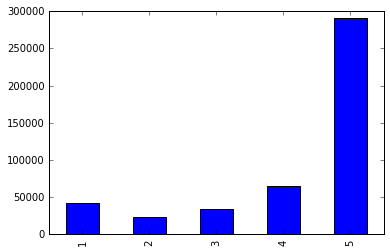
\includegraphics{reviews_x_pred}
    \caption{Distribución de reviews según puntuación. Cantidad de reviews en el eje y.}
    \label{fig:my_label}
\end{figure}

El conocimiento de la existencia de esta problemática es significativo ya que, existen algoritmos de aprendizaje que al utilizarse sobre sets de entrenamiento desbalanceados se comportaran de igual manera que un simple algoritmo que clasifique los datos según la clase mayoritaria. Esto ocurre porque la mayoría de estos algoritmos operan sobre dos premisas fundamentales:

\begin{enumerate}
    \item El objetivo es maximizar la precisión
    \item El clasificador operara sobre un set de datos de igual distribución que el de entrenamiento
\end{enumerate}

En síntesis, utilizar algoritmos de clasificación estándares sobre sets de datos desbalanceados sin ajustarlos para considerar esta característica, puede ocasionar graves errores en los resultados de la predicción. \cite{unbalanced_data}

\subsection{Palabras significativas por puntuación}
En este análisis, contamos la cantidad de apariciones de cada palabra para cada puntuación. Creemos que de esta forma podremos obtener la probabilidad de que un nuevo review del \textit{test set} pertenezca a una determinada clase (puntuación).

Comenzamos pre-procesando los campos \texttt{Summary} y \texttt{Text} con los pasos 1 a 4. Luego agrupamos estos campos según su clase y graficamos las siguientes nubes de palabras por medio de la biblioteca \texttt{wordcloud}\footnote{https://github.com/amueller/word\_cloud}. Cabe aclarar que este generador de nubes provee una lista de \textit{stop words} que excluye del gráfico.

\begin{figure}[H]
\centering
\begin{minipage}{.5\columnwidth}
  \centering
  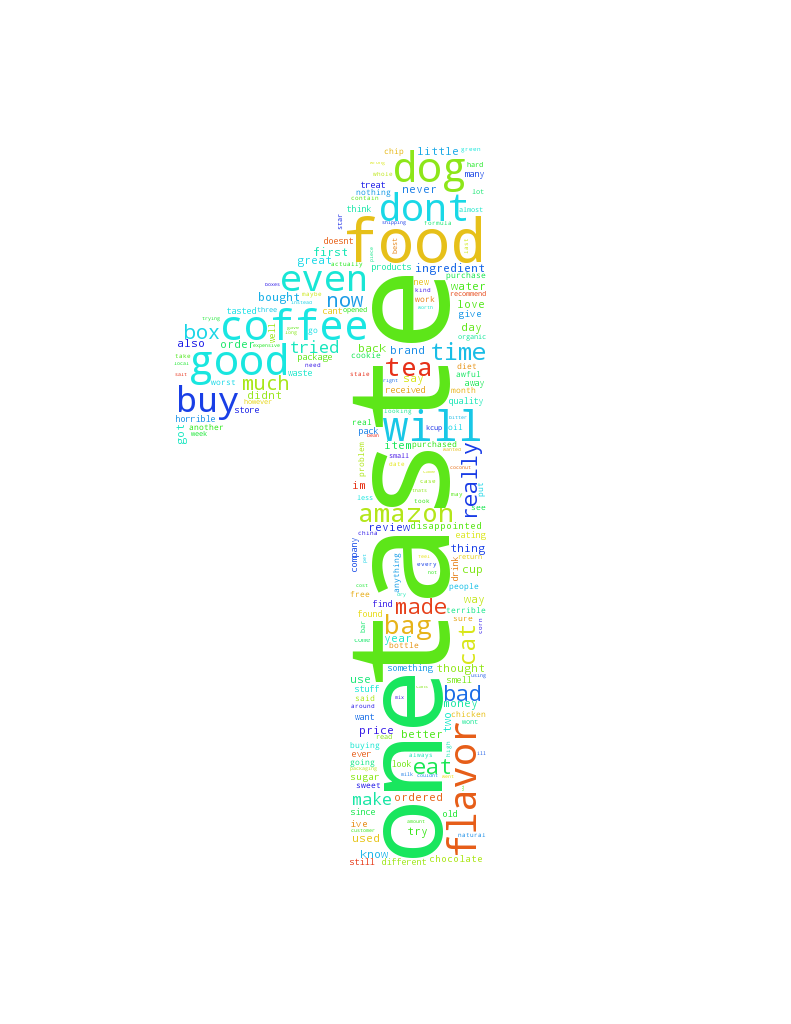
\includegraphics[width=.9\columnwidth]{wordclouds/one_cloud_scaled}
  \captionof{figure}{Nube de palabras para clase 1}
  \label{fig:my_label}
\end{minipage}%
\begin{minipage}{.5\columnwidth}
  \centering
  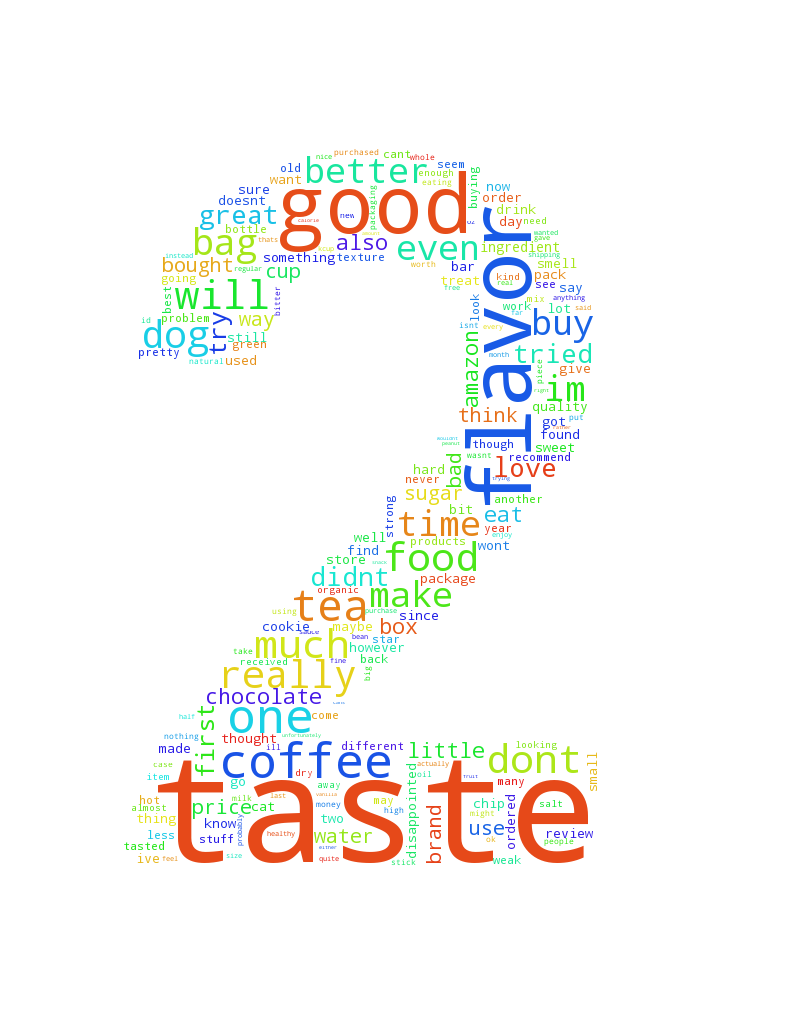
\includegraphics[width=.9\columnwidth]{wordclouds/two_cloud_scaled}
  \captionof{figure}{Nube de palabras para clase 2}
  \label{fig:my_label}
\end{minipage}
\end{figure}

\begin{figure}[H]
\centering
\begin{minipage}{.5\columnwidth}
  \centering
  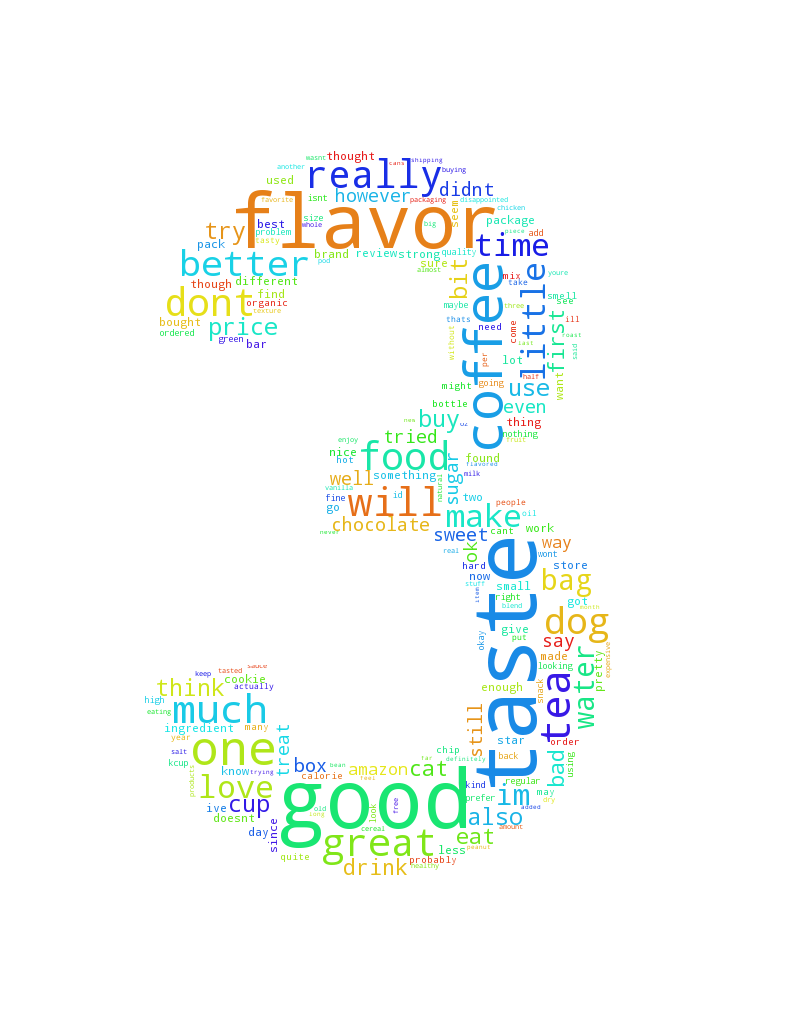
\includegraphics[width=.9\columnwidth]{wordclouds/three_cloud_scaled}
  \captionof{figure}{Nube de palabras para clase 3}
  \label{fig:my_label}
\end{minipage}%
\begin{minipage}{.5\columnwidth}
  \centering
  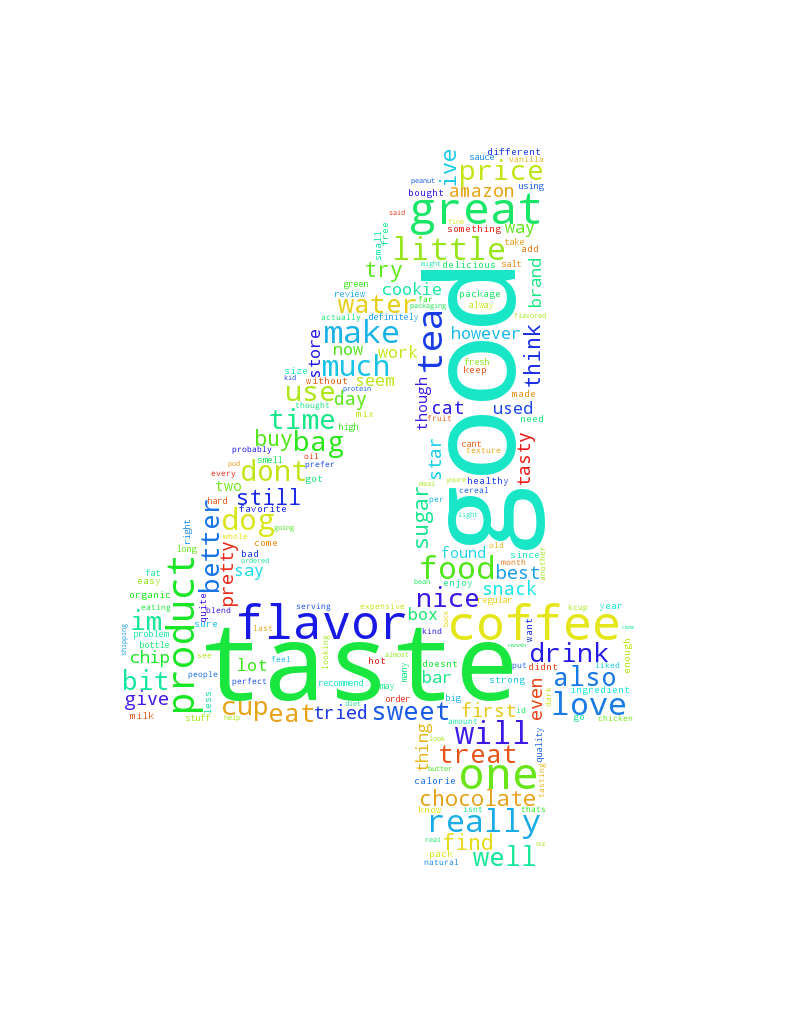
\includegraphics[width=.9\columnwidth]{wordclouds/four_cloud_scaled}
  \captionof{figure}{Nube de palabras para clase 4}
  \label{fig:my_label}
\end{minipage}
\end{figure}

\begin{figure}[H]
\centering
  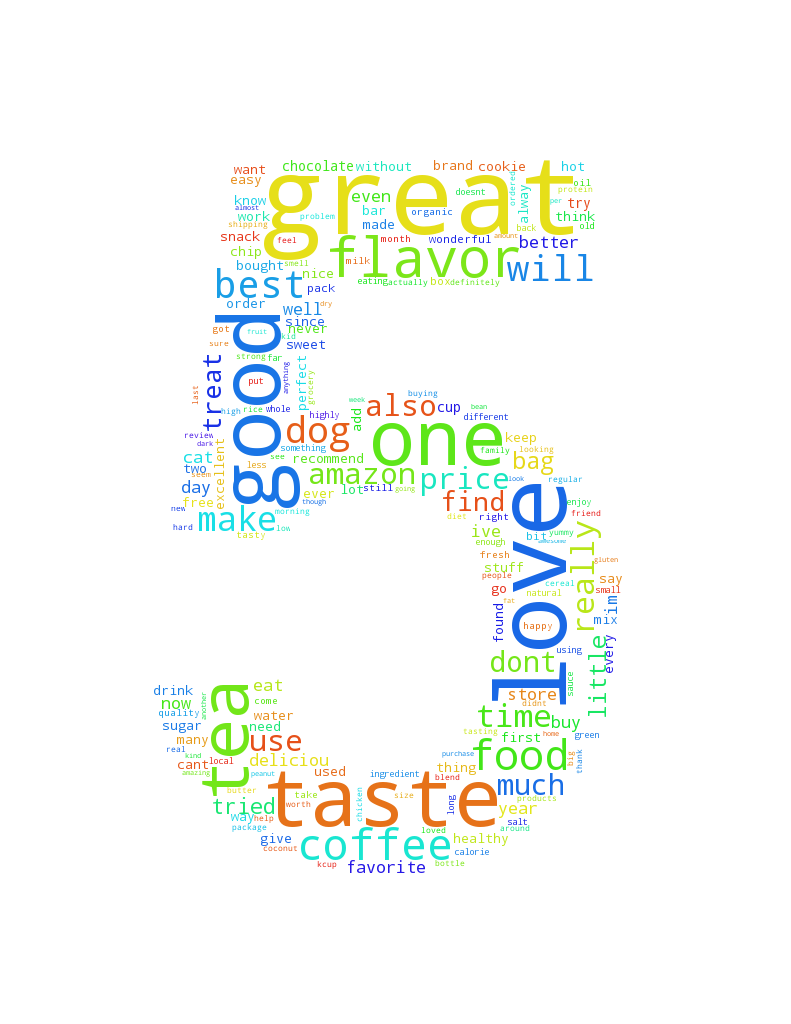
\includegraphics[width=.5\columnwidth]{wordclouds/five_cloud_scaled}
  \captionof{figure}{Nube de palabras para clase 5}
  \label{fig:my_label}
\end{figure}

Observamos que varias de las palabras predominantes son las mismas para todas las clases (Por ejemplo, \textit{taste}, \textit{flavor}, \textit{good}, son grandes en todas las nubes). Procedimos a calcular algunas probabilidades de la forma: 

\begin{equation}
    p_{palabra} = \frac{apariciones}{total}
\end{equation}

Siendo \textbf{apariciones} la cantidad de apariciones de la palabra en las \textit{reviews} de la clase x y \textbf{total} la cantidad total de palabras utilizadas para las \textit{reviews} de la clase x.

A continuación graficamos los resultados:
\begin{figure}[H]
\centering
  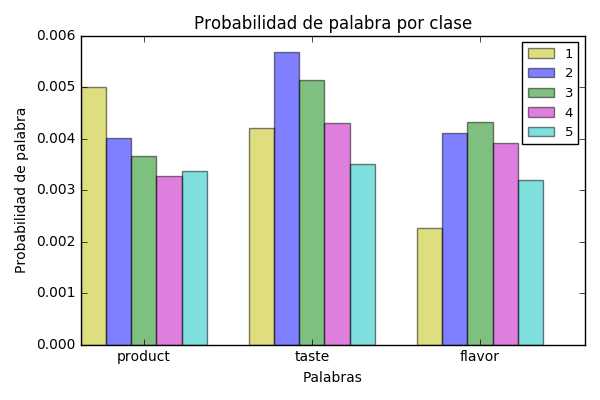
\includegraphics[width=\columnwidth]{palabras_probables}
  \captionof{figure}{Probabilidad de palabra por clase para palabras probables en todas las clases}
  \label{fig:my_label}
\end{figure}

Finalmente, comparamos la visualización anterior con una de probabilidades para palabras predominantes por clase, como por ejemplo; \textit{love} que sólo es grande en la nube clase 5.
\begin{figure}[H]
\centering
  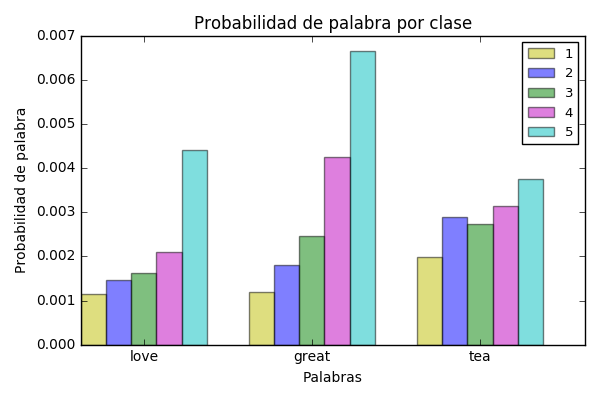
\includegraphics[width=\columnwidth]{palabras_poco_probables}
  \captionof{figure}{Probabilidad de palabra por clase para palabras probables en \textit{reviews} de clase 5}
  \label{fig:my_label}
\end{figure}

Se observa como, en el primer gráfico, ninguna barra se despega mucho de las demás, mientras que en el segundo, la barra de clase 5 supera ampliamente al resto de las clases excepto en la palabra \textit{tea}, que aunque parece predominante sólo en la nube 5, es probable que se presente en \textit{reviews} de cualquier clase.

\subsection{Entradas repetidas}
A medida que fuimos explorando el \textit{training set}, nos dimos cuenta de la existencia de \textit{reviews} repetidas. Para contabilizarlas de forma eficiente escribimos un \textit{script} en \texttt{PySpark}. A partir del mismo y con el set de entrenamiento original (sin pre-procesamiento), encontramos 48618 \textit{reviews} que poseen repeticiones (Campos \texttt{Summary}, \texttt{Text} y \texttt{Prediction} idénticos) y un total de 129432 copias de ellas. Todas las entradas respetan la unicidad del campo \texttt{Id} y, por lo que pudimos explorar, fueron escritas por el mismo usuario en el mismo momento (Mismo \texttt{UserId}, \texttt{UserName} y \texttt{Time}). Difieren en \texttt{HelpfulnessNumerator}, \texttt{HelpfulnessDenominator} y, sorprendentemente, en \texttt{ProductId}.\\ 
En conclusión, tendremos en cuenta a la hora de proponer una solución la posibilidad de recortar estas entradas repetidas, ya que en caso de no utilizar los \textit{features} \texttt{ProductId} y \texttt{Helpfulness} podemos reducir nuestro set de entrenamiento un $129432/454760 * 100 = 28.4 \% $

Además de encontrar entradas repetidas en el set de train pueden haber reviews en el set de test idénticos a uno o mas reviews del otro set. Para optimizar la predicción en este caso, podemos agrupar los reviews por su \texttt{minhash} así al compararlos pasamos de un problema de $O(n^2)$ a uno de $O(n)$. El \texttt{minhash} se calcula a partir de aplicarle una función de hashing a cada shingle del texto y quedándonos con el mínimo. 

\iffalse
\subsection{Distribución de las puntuaciones por producto en promedio, y ver si hay casos anómalos}
\hl{Se analiza el set de datos con graficos como finger 1}
\fi


\section{Investigación}

\iffalse
\subsection{Standford algorithm}
\hl{Agregar Fuente}

Este algoritmo fue creado para poder separar en frases un texto. Esto puede ser importante ya que al analizar las reviews seria imperioso poder dividir las mismas en muchas features. 

Una primera aproximación podría ser separar las reviews en palabras, no obstante esto no es siempre algo útil ya que varias palabras pueden tener significados antagónicos dependiendo de si se combinan con otras palabras o no. Un ejemplo es el siguiente, ``I like ...``, es seguramente algo positivo, mientras que ``I didn't like ...`` es seguramente algo negativo, es decir que si utilizamos sólo las palabras, en ambos aparece la palabra ``like``, sin embargo esto no quiere decir que las dos sean positivas, ya que en el segundo ejemplo se combina con un ``didn't`` adelante. Para solucionar esto, se puede dividir el texto en bi-gramas o tri-gramas y considerar cada n-grama como un feature. Así el bigrama ``not like`` es un feature que expresa realmente lo que el usuario quiso decir. 

%También deberíamos sacar signos de puntuación y \textit{stopwords} que son palabras que no agregan características al review como por ejemplo "a", "I", "mine", "the", "that", etc .

%Aqui podemos encontrar una lista de "stop words" http://xpo6.com/list-of-english-stop-words/ en formato csv facil de leer.

%Tambien se puede pasar todas las palabras a minusculas y aplicarles un proceso de stemming que significa convertirlas a su palabra raiz para que sea mas facil el aprendizaje.

\fi

\subsection{Perceptrón}

Perceptrón es un algoritmo de aprendizaje supervisado para clasificadores binarios y de tipo lineal.

Para este algoritmo se utiliza un vector de \textbf{n} dimensiones, siendo \textbf{n} igual al total de palabras sin repetir en el diccionario del set de datos. Así cuando un review es leído va a crearse un vector con un 1 en las dimensiones que aparecen. Por ejemplo si el universo de palabras es: U = ('organización', 'de', 'datos') y el review contiene las palabras: j = ('de', 'datos') el vector \textbf{x} va a quedar definido como x = (0,1,1). También se debe definir un vector de pesos \textbf{w} de \textbf{n} dimensiones, el cual generalmente comienza con valores iguales a 0 (cero): w = (0,0,0). Así para cada fila (\textbf{j}) leída del set de datos se debe calcular la predicción ($y_{j}$) con una función a definir. Por lo tanto, la ecuación resultante seria:

\begin{equation*}
    y_j = f[w_0 x_{j,0} + w_1 x_{j,1} + w_2 x_{j,2}]
\end{equation*}

Una vez calculado dicho valor, se debe actualizar el vector de pesos con la formula: 

\begin{equation*}
     w_{i} = w_{i}+(d_{j} - y_{j}) x_{j,i} 
\end{equation*}

para las dimensiones $0\leq i\leq n.$ Con $d_{j}$ el valor a predecir.

Luego se deben repetir estos dos últimos pasos hasta llegar a un error establecido o una cierta cantidad de iteraciones.

Si bien es un algoritmo diseñado para trabajar con dos clases, puede generalizarse para clasificar mas clases. Incluso en problemas de clasificación de textos. Sin embargo, según los resultados vistos en problemas similares al expuesto en el presente trabajo, este método no resulta ser el mas preciso en comparación con otros algoritmos utilizados.\cite{pcptron}

\subsection{Red multicapa}
Una red multicapa utiliza el concepto de los perceptrones donde cada perceptrón es una neurona de una red que
conecta varias de estas neuronas. Una red multicapa se puede visualizar de la siguiente manera.

\begin{figure}[H]
\centering
  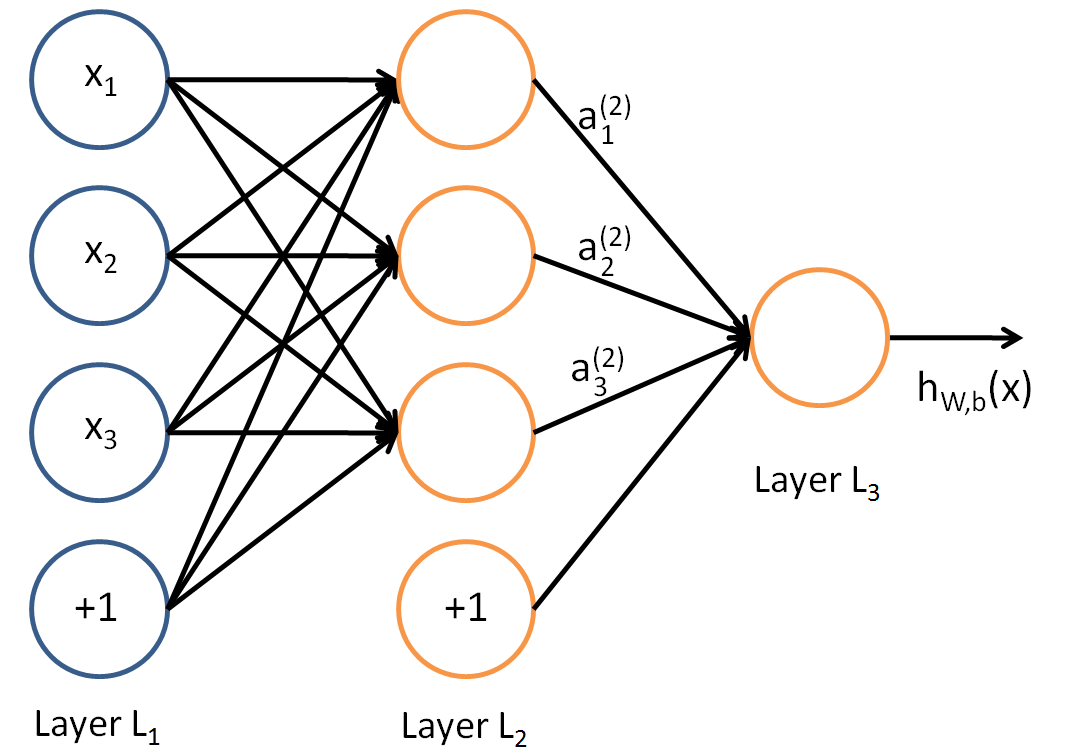
\includegraphics[width=\columnwidth]{red_neuronal.png}
  \captionof{figure}{Red Neuronal}
  \label{fig:my_label}
\end{figure}

Donde la primer capa es la \textbf{Input layer} que deriva la información que llega de \textit{input} y la reparte en la
siguiente capa. Las subsiguientes capas son las \textbf{Hidden layers} donde se van distribuyendo los datos capa a capa
y finalmente se llega al \textbf{Output layer} que es el resultado. En la imagen presentada el \textit{output layer} es una sola neurona, sin embargo no es necesario, podría haber $n$ neuronas en el \textit{output layer}.

En la siguiente sección, describimos algunos de los métodos de aprendizaje para las redes neuronales:

\subsubsection{Modelos de aprendizaje}
Los modelos de dividen en \textbf{Algoritmos de aprendizaje}
{\begin{itemize}
    \item \textbf{Corrección de error}
    \item \textbf{Aprendizaje Hebbiano}
    \item \textbf{Aprendizaje Competitivo}
\end{itemize}
y, por otro lado, \textbf{Paradigmas de aprendizaje}: 
{\begin{itemize}
    \item \textbf{Aprendizaje Supervisado} 
    \item \textbf{Aprendizaje reforzado}
    \item \textbf{Aprendizaje no supervisado}
\end{itemize}

El \textbf{Aprendizaje Supervisado} es el tipo de entrenamiento en el cual se provee al sistema con información de las
entradas al igual que se proveen las salidas esperadas o destinos correspondientes a dichas entradas a modo que el
sistema tenga los destinos como punto de referencia para evaluar su desempeño en base a la diferencia de estos valores y
modificar los parámetros libres en base a esta diferencia.\cite{udlap}

En un \textbf{Aprendizaje no supervisado} los parámetros libres del sistema son modificados únicamente en base a las
entradas del sistema de manera que aprenden a categorizar las entradas y clasificarlas sin necesidad de una
referencia.

La \textbf{Regla delta} o \textbf{Algoritmo de corrección de error} se refiere al modelo de aprendizaje que se basa en
minimizar una función de error en relación a los parámetros libres del sistema.
Una vez definida la función de costo a minimizar la corrección de error es un problema estrictamente de optimización.

El \textbf{Aprendizaje Hebbiano} indica que las conexiones entre las neuronas de entrada activas y las neuronas de
salida activas se refuerzan durante el entrenamiento: coincidencias entre actividad de entrada y actividad de salida se
intensifican. Mientras que las conexiones entre neuronas de entrada inactivas y neuronas de salida (Activas o Inactivas)
no se refuerzan. 

Este método de aprendizaje puede ser tanto supervisado como no supervisado. Cuando es supervisado, la respuesta correcta
para el dato de entrada es introducida para cada neurona de salida, y los pesos sinápticos entre las neuronas activas se
incrementan, mientras que los pesos entre neuronas que no estén activas simultáneamente permanecen igual que estaban.

En el \textbf{Aprendizaje competitivo} suele decirse que las neuronas compiten (Y Cooperan) unas con otras con el fin de
llevar a cabo una tarea dada. Con este tipo de aprendizaje se pretende que cuando se presente a la red cierta
información de entrada, sólo una de las neuronas de salida de la red, o una por cierto grupo de neuronas, se active
(Alcance su Valor de Respuesta Máximo). Por tanto las neuronas compiten para activarse quedando finalmente una, o una
por grupo, como neurona vencedora y el resto quedan anuladas y siendo forzadas a sus valores de respuesta mínimos.

% \begin{comment}
% Las redes competitivas, son bastante eficientes para resolver problemas de clasificación, sin embargo presentan
% algunos problemas. El primero es la elección de una rata de aprendizaje que permita hallar un punto de equilibrio entre
% velocidad de convergencia y la estabilidad final de los vectores de peso. Una rata de aprendizaje cercana a cero, torna
% el aprendizaje muy lento pero garantiza que cuando un vector haya alcanzado el centro de la clase objetivo, se mantendrá
% allí indefinidamente. En contraste, una rata de aprendizaje cercana a uno genera un aprendizaje muy rápido, pero los
% vectores de peso continuarán oscilando aún después de que se haya alcanzado convergencia. La indecisión que se presenta
% al escoger la rata de aprendizaje puede ser empleada como una ventaja si se inicia el entrenamiento con una rata de
% aprendizaje alta y se decrementa en el transcurso del proceso de entrenamiento cuando sea necesario, desafortunadamente
% esta técnica no funciona si la red necesita continuamente ser adaptada a nuevos argumentos de los vectores de entrada
% (Caso en que la Red se Trabaje On-Line).

% \end{comment}


\subsection{The Hashing Trick}

También conocido como feature hashing, al igual que otros algoritmos como preceptrón, toma ventaja de la separación en \textit{tokens} del review y crea un vector de features. A cada feature, en nuestro caso a cada palabra, del vector que define una fila en el set de datos se le aplica una función de hashing $h_{1}$, que como sabemos devuelve un número. A dicho número se le aplica la función \textbf{mod d} con $d \le n$. Siendo \textbf{n} el numero de dimensiones del vector original y \textbf{d} el número de dimensiones del vector final. Así la idea es reducir el numero de dimensiones de nuestro set de datos. Esto tiene una desventaja que puede generar colisiones, es decir, textos que son distintos pero al ser hasheados parecen similares. Dicho problema se puede solucionar con una segunda función de hashing $h_{2}$ que para dimensión devuelva dos valores +1 o -1. Entonces según $h_{2}$ sea positiva o negativa se va a sumar o restar 1 a la posición indicada por $h_{1}$. Esto reduce las probabilidades de colisiones y nos permite encontrar textos similares con mayor facilidad.

Otra ventaja de este algoritmo es que el vector resultante suele ser muy disperso, por lo que guardarlo con un algoritmo adecuado puede ayudarnos a reducir mucha memoria.

Una desventaja de este algoritmo es que se pierde la interpretación de los datos.

Según las ultimas aplicaciones del hashing trick clasificando textos con funciones de hashing aleatorias y decenas de miles de columnas en el vector de salida no presenta problemas de performance, hasta incluso sin el uso de $h_{2}$.\cite{hashing_trick}


\subsection{Naïve bayes}

Naïve Bayes es una extensión de Bayes para n características, las cuales se asumen independientes.

\begin{equation*}
    P(y|x_1,..,x_n) = \frac {P(y)\prod_{i = 1}^{n} {P(x_i|y)}} {P(x_1,..,x_n)}
\end{equation*}

En donde 'y' seria la puntuación y 'x' cada feature que en nuestro caso corresponde a cada palabra. Entonces vamos a calcular a 

\begin{enumerate}
    \item P(y) como la $\frac {review-de-clase-x}{total-de-reviews}$
    \item $P(x|y)$ como la frecuencia de la palabra x en la clase y $ p_{palabra} = \frac{apariciones}{total} $ 
    \item $P(x_1,..,x_n)$ como la probabilidad de que en un review aparezcan esas palabras.
\end{enumerate}

La frecuencia de las palabras se almacena en tablas de hash durante la fase de entrenamiento. De esta forma vamos a predecir a un review con el $P(y|x_1,..,x_n)$ más grande.\cite{naive_bayes}\\

Si el clasificador se encuentra con una palabra que no ha visto antes en el set de entrenamiento, nos encontramos con un problema de probabilidad cero. La solución más simple al problema es sumar 1 a la frecuencia de cualquier palabra en cualquier contexto, a esto se lo llama \textbf{ajuste de Laplace}.\\

Una desventaja de Bayes es el overfitting, al encontrar palabras poco frecuentes que aparecen sólo en una clase, el algoritmo clasifica al documento dentro de esta clase y cree que cualquier entrada con esa palabra pertenece exclusivamente a la clase en la que la observó. Esto puede evitarse ignorando las palabras con baja frecuencia o que solo pertenecen a una clase.\cite{apunte}\\

Su ventaja principal es la capacidad de escalar grandes sets de datos sin problemas. Se pueden eliminar las palabras duplicadas de los documentos, ya que no agregan información adicional; a este tipo de algoritmo se lo llama \textbf{Bernoulli Naïve Bayes}. Incluir la presencia de una palabra en lugar de su recuento mejora la performance significativamente cuando hay muchas entradas en el set de entrenamiento.\cite{bayes_paper}

\subsection{SVM}
SVM o Support Vector Machines son modelos de aprendizaje supervisado asociados con algoritmos para resolver problemas de clasificación y regresión. SVM es particularmente útil para categorización de textos e incluso obtiene mejores resultados que otros algoritmos convencionales.\cite{svm_thorsten}

El modelo teórico de SVM es muy sencillo y puede expresarse a partir de los conceptos del modelo ``Perceptrón''. En este ultimo se buscaba un hiperplano o recta que separara a las clases que se quieren clasificar, en SVM no solo se busca dicho hiperplano si no que se pretende encontrar el mejor de ellos para realizar la clasificación. Para encontrar el hiperplano que mejor separa las clases se utiliza el concepto del ``margen'', en SVM el mejor hiperplano es aquel que maximiza el margen entre las clases.\cite{apunte} El margen es la región comprendida entre dos hiperplanos que separan los elementos. Esta región es de la mayor distancia posible mientras que los elementos continúen separados. 


Si bien SVM es introducido como un modelo para resolver problemas de clasificación lineal, es posible adaptarlo para resolver problemas en donde existen mas de dos clases, como es el caso del presente trabajo. Una de las opciones para lograr solucionar este problema es utilizar varios clasificadores lineales que separen a una de las clases con el resto, es decir que se transforma el problema de clasificación entre mas de dos clases en varios problemas de clasificación binarios independientes. Esta estrategia imposibilita la relación entre distintas clases ya que pertenecen a problemas independientes entre si.\cite{svm_crammer} Existen casos en donde SVM fue utilizado para clasificación de textos en problemas con mas de dos clases y se obtuvieron resultados satisfactorios e incluso mejores que los obtenidos con otros algoritmos. \cite{svm_thorsten}

\section{Modelos utilizados}
\subsection{Vowpal Wabbit}
Como parte de un finger exercise, realizamos predicciones sobre el test set utilizando la herramienta \textbf{Vowpal Wabbit}.\\
El proyecto Vowpal Wabbit es un sistema de aprendizaje rápido diseñado para procesar sets de datos completos que son demasiado grandes para caber en la memoria principal de una computadora.\\

Hay dos maneras de tener un algoritmo de aprendizaje rápido:
\begin{itemize}
    \item Comenzar con un algoritmo lento y acelerarlo
    \item Construir un algoritmo de aprendizaje intrínsecamente rápido
\end{itemize}
Este proyecto se basa en el segundo enfoque, y se llegó a un estado en el que puede ser útil a los demás como una plataforma para investigación y experimentación.\\

Existen varios algoritmos de optimización disponibles, siendo la base un \textit{gradient descent (GD)} disperso en una \textit{loss function} (De las múltiples disponibles).\cite{vw}\\

Antes de comenzar a predecir, pre-procesamos ambos sets de datos con los pasos 1 a 6 y tomamos exclusivamente los features \texttt{Summary}, \texttt{Text}, \texttt{Prediction} y \texttt{Id} (Este último como tag única para cada review) pasándolos al formato de entrada pedido por vw.\\

Comenzamos entrenando con los siguientes flags\cite{vw_flags}:
\begin{itemize}
    \item \texttt{--passes 300}: Realiza 300 pasadas sobre el training set
    \item \texttt{--ngram 7}: Crea 7-gramas
    \item \texttt{-b 24}: Utiliza hashes de 24 bits (Por defecto son 18)
    \item \texttt{--ect 5}: Utiliza \textit{error correcting tournament}, notifica la existencia de 5 labels posibles y pide que se elija una por entrada
\end{itemize}
logrando predecir con un puntaje de \texttt{0.51373} en Kaggle.\\

En un segundo intento, entrenamos con los flags:
\begin{itemize}
    \item \texttt{--passes 300}: Explicado anteriormente
    \item \texttt{--ngram 2}: Crea bigramas
    \item \texttt{-b 24}: Explicado anteriormente
    \item \texttt{--skips 2}: Genera saltos de a bigramas
    \item \texttt{--decay\_learning\_rate=.95}: Establece un factor de decaimiento, entre pasadas, para la tasa de aprendizaje
    \item \texttt{--ftrl}: Utiliza la optimización \textit{Follow the (Proximal) Regularized Leader}
\end{itemize}
Logrando un puntaje final de \texttt{0.41703} en Kaggle.

\subsection{Dynamic vector prediction}

Inspirados en la charla de las jaiio y de la manera en que facebook hacia sentiment analisis, propusimos un algoritmo similar que lo bautizamos Dynamic vector prediction.

El algorimo consiste en armar una tabla de la forma palabra:cardinalidad de la palabra por cada predicción. Por ejemplo, en el caso de la predicción 1.

\begin{lstlisting}[firstnumber=1]
    {
    "tast":22508,
    "br":22305,
    "like":21614,
    "product":21051,
    "one":15308,
    "food":14724
    .
    .
    .
    }
\end{lstlisting}

Esto se genera recorriendo todos los reviews y de una misma predicción y sumando 1 por cada palabra. Ésta tabla de frecuencias seria el equivalente al aprendizaje.

Para poder predecir un review por ejemplo ``The food was awful'' 

Se hace un split lo cual queda [``The'', ``food'' ,  ``was'',  ``awful'' ]. Teniendo esto que llamaremos, la referencia, se genera un vector, llamado vector dinámico con la cardinalidad de cada palabra. Es decir, si alguna palabra se repitiera, no estaría duplicada en las referencias pero si aumentaría la cardinalidad en el vector dinámico. En este caso el vector dinámico quedaría de la siguiente forma. [1, 1, 1, 1]. 

Teniendo las tablas de frecuencias de las 5 predicciones, se hace lo mismo con las palabras de referencia. Por ejemplo, si ``The'' tiene cardinalidad 10000, ``food'' 1500,``was'' 10000 y ``awful''500, en la predicción 1 entonces el vector dinámico es [10000, 1500, 1000, 500]. Esto se repite con todas las predicciones.

A esta altura se generaron 6 vectores dinámicos, el de la review + las 5 predicciones. Para poder comprar todos los reviews de la misma forma, sabiendo que el set de datos está desbalanceado, se procede a normalizar los 6 vectores.

Finalmente se calcula la distancia coseno entre la review contra todas las predicciones y se queda con la menor. Esto define a cuál se parece más y esa es la predicción.


Los resultados de éste algoritmo se probaron con tres distancias distintas y se hizo un post en Kaggle con la mejor de ellas. Basándonos en cuánto se ajustaba al train set.

Con la distancia del coseno los resultados fueron 377 predicciones correctas con respecto a mil. Con la Euclideana fueron 345. Mientras que con Jaccard 77.

Se obtuvo una puntuación de \texttt{5.06451} en Kaggle, por lo que concluimos en que el algoritmo no es bueno para este tipo de problema.

\section{Modelo a implementar}%Modelo a implementar? Propuesta de resolucion? Es mas que un algoritmo lo que proponemos Solucion a implementar?

\subsection{Pre-procesamiento}
Para la solución a implementar se decidió utilizar los pasos 1 a 4 sobre los sets training y test, obviando la eliminación de stopwords, ya que desempeñan una función importante a la hora de entender los sentimientos de los usuarios.

En segundo lugar, se propone realizar un manejo de las negaciones. Al utilizar cada palabra como un feature, la palabra ``good'' en la frase ``not good'' contribuirá a un sentimiento positivo en lugar de a uno negativo, debido que la presencia de ``not'' no se tiene en cuenta. Para resolver este problema se escribirá un \textit{script} que transforme una palabra seguida de un ``not'' o ``n't'' en ``not\_'' + palabra. Las palabras a negar se detectan con una variable de estado, cuando esta es verdadera, a todas las palabras leídas se les antepondrá la negación. La variable vuelve a su valor inicial cuando se encuentra un signo de puntuación u otra negación. %recordar cambiar el preprocess para que deje ' y .

\subsection{Procesamiento}
Previo al entrenamiento del modelo elegido, se deberá preparar el set de acuerdo a los requisitos del algoritmo. Además se determinará qué campos serán incluidos para realizar el entrenamiento, en base a lo explicado en apartados anteriores.

El procesamiento propuesto consiste en construir una matriz compuesta por los Id's de los productos, su puntaje y todas las palabras halladas en los campos ``Summary'' y ``Text'' de  todas las reviews. Cada fila de esta matriz corresponde a un review individual. Cada una de las palabras corresponderá a un atributo y tendrán un valor entre 0 y N dependiendo de la cantidad de veces que dicha palabra aparezca en la review. A continuación se presenta un ejemplo de la matriz:

\begin{table}[H]
    \centering
    \begin{tabular}{|ccccc|}
    \hline
     ProductId& Prediction & good & not\_good & taste \\ \hline \hline
     1 & 4 & 3 & 0 & 1 \\
     2 & 1 & 0 & 2 & 2 \\
     3 & 2 & 1 & 3 & 0\\
     4 & 2 & 0 & 1 & 0\\ \hline
    \end{tabular}
    \caption{}
\end{table}

Dado que la gran cantidad de palabras existentes tiene como consecuencia que las matrices tengan una dimensión demasiado grande, se filtrarán las palabras en base a su ocurrencia. Sabiendo que la cardinalidad de las palabras por predicción se distribuye como una ley de potencias, se podrá encontrar algún porcentaje empírico de palabras, las más relevantes, que se utilizarán para entrenar. Y siendo ésta distribución una ley de potencias, dicha relación es invariante a la escala, es decir, que para todas las predicciones (independientemente de la cantidad de reviews que tengan) se podrá usar la mismo proporcionalidad.

Otra forma de reducir éste número es aplicarle the hashing trick a las palabras y así poder reducir las dimensiones de la matriz. Se probará si hace falta aplicarle the hashing trick, y si hiciera falta, cuán costoso és. 

\subsection{Predicción}
El modelo que se utilizará para predecir el puntaje de los reviews será SVM, como ya se explicó, SVM es un algoritmo especialmente útil para clasificación de textos. Este modelo puede ser utilizado para problemas no lineales, como es el caso del presente trabajo \cite{svm_crammer} y se cuenta con evidencia empírica de que obtiene mejores resultados que otros algoritmos para problemas de clasificación no lineales. \cite{svm_thorsten}

Según lo investigado, SVM no funciona bien para sets de datos desbalanceados\cite{quora}, lo cual es nuestro caso (como fue detallado en el análisis del set de datos). Para solucionar este problema se pueden usar dos aproaches; Una solución posible es balancear el set de datos, recortándolo aleatoriamente o aprovechando a sacar las entradas repetidas. Por otro, si esto último no funciona, optaremos por cambiar el predictor por otro, como un perceptrón multicapa.

\iffalse
Primero hay que filtrar los datos buscando anomalias en ellos, como por ejemplo reviews repetidas, dos reviews sobre un producto del mismo usuario y casos en los que esta muy desbalanceada la clasificacion para un producto puede surgir de un error de tipeo por parte del usuario.

Luego podemos sacar los campos que no son relevantes para nuestro problema como por ejemplo los campos "Time", "Profile Name", "Id". Despues de haber hecho el analisis anterior tambien podriamos sacar los campos "ProductId" y "UserId". \hl{Que hacemos con el Helpfulness numerator y denominator?}
\fi

\pagebreak

\section{Bibliografía}
\bibliography{ref}
\bibliographystyle{unsrt}
\end{document}
